
%(BEGIN_QUESTION)
% Copyright 2013, Tony R. Kuphaldt, released under the Creative Commons Attribution License (v 1.0)
% This means you may do almost anything with this work of mine, so long as you give me proper credit

Interpret the pressure measurement displayed by this water-filled U-tube manometer, assuming each division on the scale is equal to 1 inch:

$$\epsfysize=7in \includegraphics[width=15.5cm]{i02821x01.eps}$$

Express your answer both in {\it inches of water column} ("WC) and {\it pounds per square inch} (PSI):

\vskip 10pt

$P$ = \underbar{\hskip 50pt} "WC

\vskip 10pt

$P$ = \underbar{\hskip 50pt} PSI


\underbar{file i02821}
%(END_QUESTION)





%(BEGIN_ANSWER)

$P$ = \underbar{\bf 22} "WC

\vskip 10pt

$P$ = \underbar{\bf 0.795} PSI
 
%(END_ANSWER)





%(BEGIN_NOTES)


%INDEX% Measurement, manometer reading

%(END_NOTES)


